\documentclass[12pt,a4paper,openany]{report}
\usepackage[T1]{fontenc}
\usepackage{lmodern}
\usepackage[margin=1in]{geometry}
\usepackage{tabularx}
\usepackage{booktabs}
\usepackage{titlesec}
\titlespacing*{\chapter}{0pt}{0pt}{18pt}
\titlespacing*{\section}{0pt}{8pt}{2pt}
\usepackage{tikz}
\usetikzlibrary{positioning,calc,arrows.meta}

\definecolor{apexfill}{HTML}{DCE6F1}
\definecolor{apexline}{HTML}{2F5496}
\definecolor{subfill}{HTML}{F2F2F2}
\definecolor{subline}{HTML}{666666}
\definecolor{cabfill}{HTML}{BDD7EE}
\definecolor{cabline}{HTML}{1F4E79}
\definecolor{mosfill}{HTML}{FCE4D6}
\definecolor{mosline}{HTML}{C55A11}
\definecolor{cmred}{HTML}{C00000}
\hyphenation{Chancellorship direction}

\tikzset{
  hroot/.style={draw=apexline, fill=apexfill, rounded corners=4pt,
                line width=0.8pt, text width=3.6cm, align=center,
                minimum height=1.25cm, font=\bfseries,
                execute at begin node={\hyphenpenalty=10000\relax}},
  hlvl/.style={draw=apexline!70, fill=apexfill!60, rounded corners=3pt,
               line width=0.7pt, text width=3.2cm, align=center,
               minimum height=1.1cm, font=\small,
               execute at begin node={\hyphenpenalty=10000\relax}},
  hsub/.style={draw=subline, fill=subfill, rounded corners=3pt,
               line width=0.6pt, text width=2.7cm, align=center,
               minimum height=1.0cm, font=\small},
  hleaf/.style={draw=subline, fill=subfill!75, rounded corners=3pt,
                line width=0.6pt, text width=2.7cm, align=center,
                minimum height=0.9cm, font=\footnotesize,
                execute at begin node={\hyphenpenalty=10000\relax}},
  cabbox/.style={draw=cabline, fill=cabfill, rounded corners=3pt,
                 line width=0.8pt, text width=3.4cm, align=center,
                 minimum height=1.1cm, font=\bfseries\small},
  mosbox/.style={draw=mosline, fill=mosfill, rounded corners=3pt,
                 line width=0.8pt, text width=3.4cm, align=center,
                 minimum height=1.1cm, font=\bfseries\small},
  minbox/.style={draw=subline, fill=subfill!70, rounded corners=2pt,
                 line width=0.5pt, text width=3.4cm, align=center,
                 minimum height=0.9cm, font=\scriptsize,
                 execute at begin node={\hyphenpenalty=10000\relax}},
  hlink/.style={draw=black!65, line width=0.7pt}
}

\begin{document}

% ---------------------------------------------------------------- title page
\begin{titlepage}
  \centering
  \vspace*{5cm}
  {\Huge\bfseries Jharkhand State Administration\par}
  \vspace{0.8cm}
  {\Large Administrative Hierarchy\par}
  \vfill
\end{titlepage}

% ---------------------------------------------------------------- chapter 1
\begin{center}
\resizebox{\textwidth}{!}{%
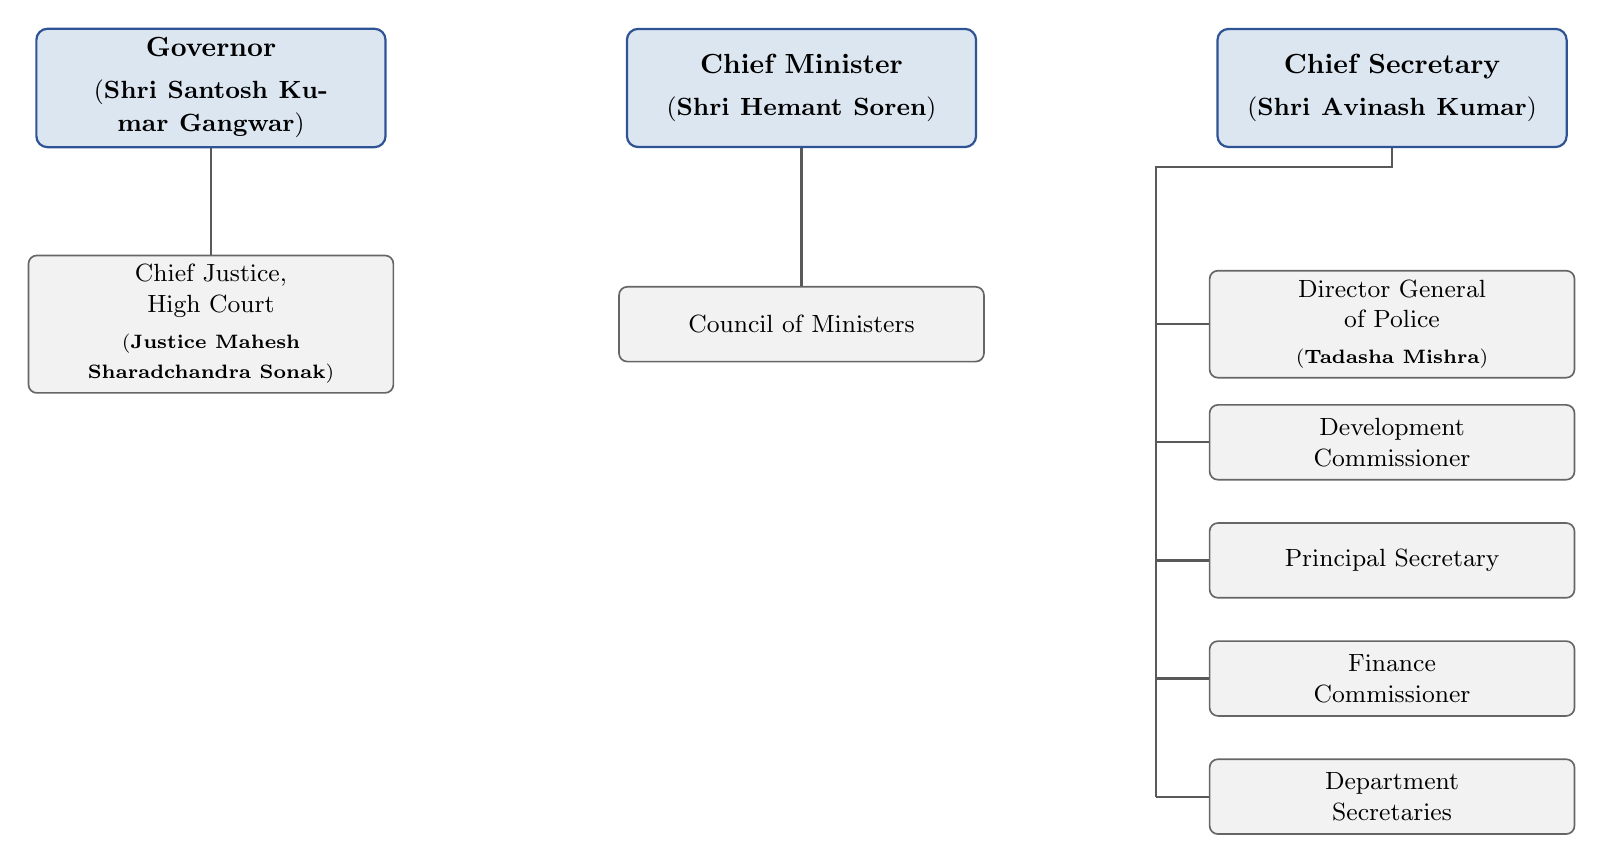
\begin{tikzpicture}[
  apex/.style={draw=apexline, fill=apexfill, rounded corners=4pt,
               line width=0.8pt, text width=4.2cm, align=center,
               minimum height=1.5cm, font=\bfseries},
  sub/.style={draw=subline, fill=subfill, rounded corners=3pt,
              line width=0.6pt, text width=4.4cm, align=center,
              minimum height=0.95cm, font=\small},
  link/.style={draw=black!65, line width=0.8pt}
]

% ---- apex level -----------------------------------------------------------
\node[apex] (gov) at (-7.5,0)
  {Governor\\[3pt]{\normalfont\small (\textbf{Shri Santosh Kumar Gangwar})}};

\node[apex] (cm) at (0,0)
  {Chief Minister\\[3pt]{\normalfont\small (\textbf{Shri Hemant Soren})}};

\node[apex] (cs) at (7.5,0)
  {Chief Secretary\\[3pt]{\normalfont\small (\textbf{Shri Avinash Kumar})}};

% ---- second level ---------------------------------------------------------
\node[sub] (cj) at (-7.5,-3.0)
  {Chief Justice,\\High Court\\[2pt]{\scriptsize (\textbf{Justice Mahesh Sharadchandra Sonak})}};

\node[sub] (com) at (0,-3.0)
  {Council of Ministers};

\node[sub] (dgp) at (7.5,-3.0)
  {Director General\\of Police\\[2pt]{\scriptsize (\textbf{Tadasha Mishra})}};

\node[sub] (dc) at (7.5,-4.50) {Development\\Commissioner};
\node[sub] (ps) at (7.5,-6.00) {Principal Secretary};
\node[sub] (fc) at (7.5,-7.50) {Finance\\Commissioner};
\node[sub] (ds) at (7.5,-9.00) {Department\\Secretaries};

% ---- links ----------------------------------------------------------------
\draw[link] (gov.south) -- (cj.north);
\draw[link] (cm.south)  -- (com.north);

\coordinate (busTop) at (4.5,-1.0);
\coordinate (busBot) at (4.5,-9.00);
\draw[link] (cs.south) -- (7.5,-1.0) -- (busTop) -- (busBot);
\foreach \n/\y in {dgp/-3.0, dc/-4.50, ps/-6.00, fc/-7.50, ds/-9.00}
  \draw[link] (4.5,\y) -- (\n.west);

\end{tikzpicture}%
}
\end{center}

\section*{How These Apex Level Inter-related}

\noindent{\footnotesize
\renewcommand{\arraystretch}{1.32}%
\begin{tabularx}{\textwidth}{@{}>{\raggedright\arraybackslash}p{3.5cm} X >{\raggedright\arraybackslash}p{3.2cm}@{}}
\toprule
\textbf{Pair} & \textbf{Nature of relation} & \textbf{Basis} \\
\midrule
Governor $\leftrightarrow$ Chief Minister &
Governor appoints the CM; ministers are appointed on the CM's advice; Governor acts on the aid and advice of the Council of Ministers; CM is the channel of communication and keeps the Governor informed. &
Arts.\ 163, 164, 167 \\
\addlinespace[4pt]
Governor $\leftrightarrow$ Chief Minister (discretion) &
May reserve a Bill, recommend President's Rule, or exercise discretion in a hung Assembly. &
Arts.\ 200, 356 \\
\addlinespace[4pt]
Chief Minister $\rightarrow$ Chief Secretary &
CM/Cabinet directs policy; CS is principal adviser, Secretary to the Cabinet, and head of the IAS bureaucracy; appointed by the Cabinet Appointment Committee. &
Non-constitutional \\
\addlinespace[4pt]
Governor $\leftrightarrow$ Chief Secretary &
Liaison, protocol and briefing only; no command---the CS answers to the elected government. &
Administrative practice \\
\addlinespace[4pt]
Chief Secretary $\rightarrow$ Department Secretaries &
Converts Cabinet decisions into implementation; supervises departmental secretaries and field administration. &
Service rules and executive instructions \\
\bottomrule
\end{tabularx}}


\noindent\textbf{Flow of authority:} Governor (appoints, advises) $\leftrightarrow$ Chief Minister (directs) $\rightarrow$ Chief Secretary (implements) $\rightarrow$ Department Secretaries $\rightarrow$ field administration.

\noindent\textbf{Accountability:} CM to the Assembly; CS to the CM/Cabinet; Governor to the President.

% ================================================================ Governor
\newpage
\section*{Hierarchies under the Governor}

\begin{center}
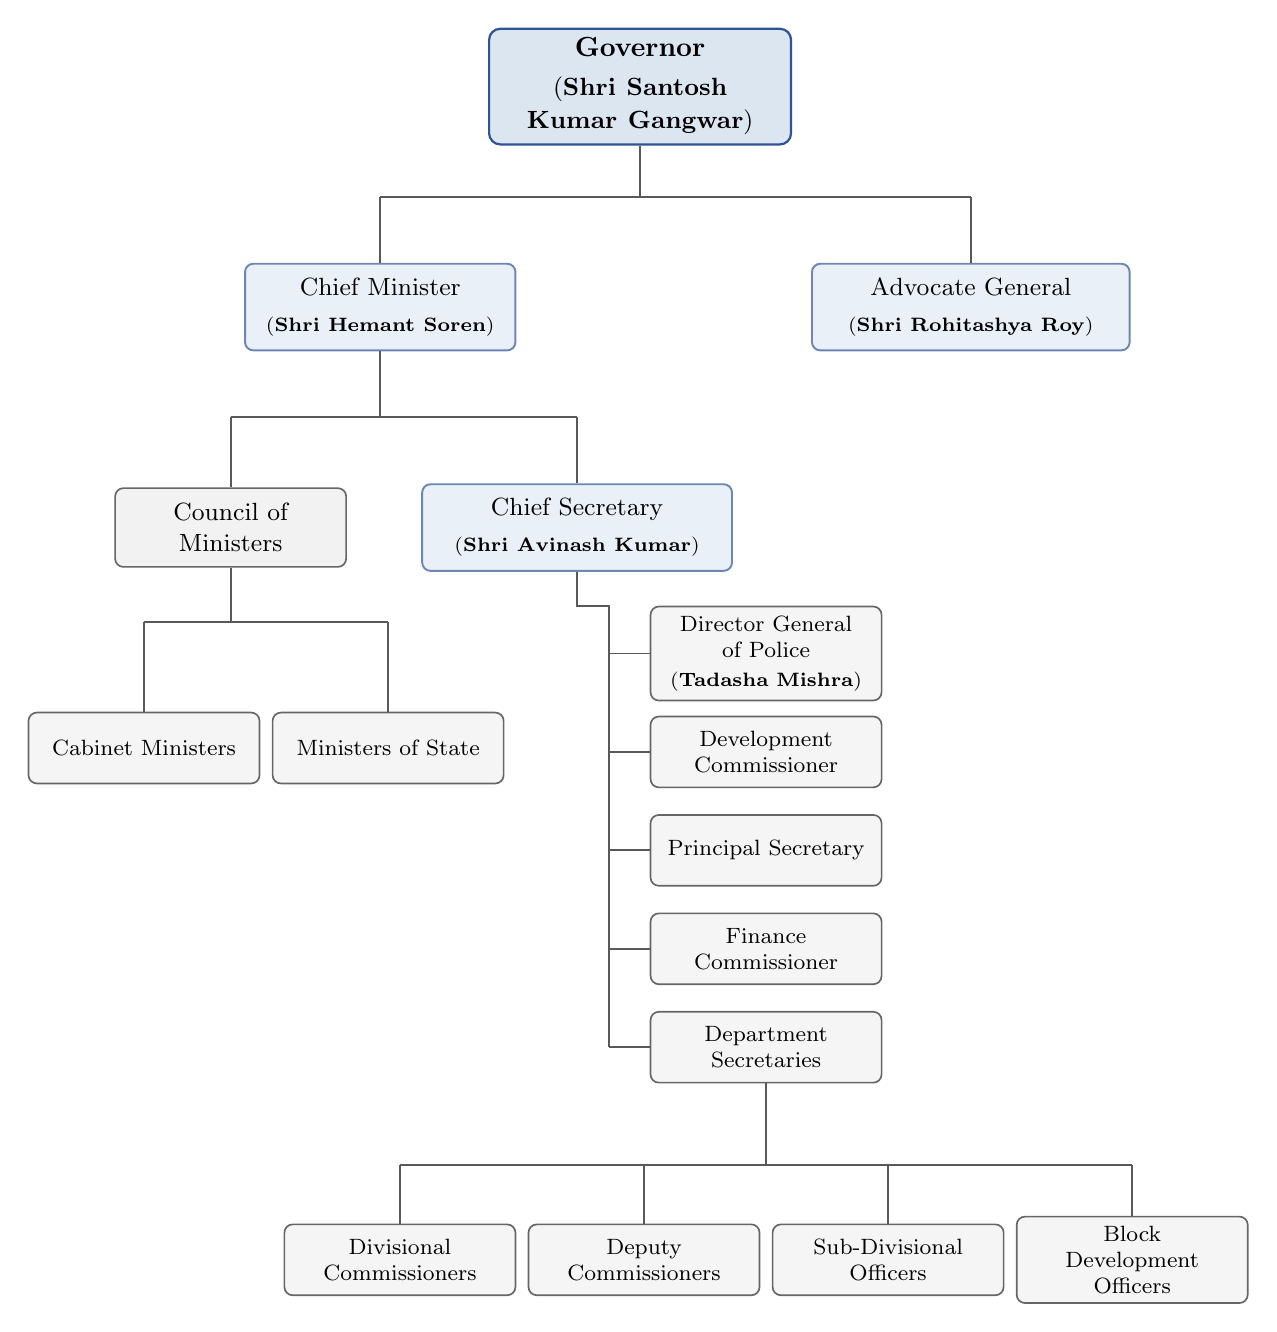
\begin{tikzpicture}
  \node[hroot] (gov) at (0,0)
    {Governor\\[2pt]{\normalfont\small (\textbf{Shri Santosh Kumar Gangwar})}};
  \node[hlvl] (cm) at (-3.3,-2.8)
    {Chief Minister\\[2pt]{\normalfont\scriptsize (\textbf{Shri Hemant Soren})}};
  \node[hlvl, text width=3.8cm] (ag) at (4.2,-2.8)
    {Advocate General\\[2pt]{\normalfont\scriptsize (\textbf{Shri Rohitashya Roy})}};

  \node[hsub] (council) at (-5.2,-5.6) {Council of Ministers};
  \node[hlvl, text width=3.7cm] (cs) at (-0.8,-5.6)
    {Chief Secretary\\[2pt]{\normalfont\scriptsize (\textbf{Shri Avinash Kumar})}};

  \node[hleaf] (cab) at (-6.3,-8.4) {Cabinet Ministers};
  \node[hleaf] (mos) at (-3.2,-8.4) {Ministers of State};

  \node[hleaf] (dgp) at (1.6,-7.2)
    {Director General\\of Police\\[1pt]{\scriptsize (\textbf{Tadasha Mishra})}};
  \node[hleaf] (dev) at (1.6,-8.45) {Development\\Commissioner};
  \node[hleaf] (ps)  at (1.6,-9.7)  {Principal Secretary};
  \node[hleaf] (fc)  at (1.6,-10.95) {Finance\\Commissioner};
  \node[hleaf] (ds)  at (1.6,-12.2) {Department\\Secretaries};

  \node[hleaf] (fdiv) at (-3.05,-14.9) {Divisional\\Commissioners};
  \node[hleaf] (fdc)  at (0.05,-14.9)  {Deputy\\Commissioners};
  \node[hleaf] (fsdo) at (3.15,-14.9)  {Sub-Divisional\\Officers};
  \node[hleaf] (fbdo) at (6.25,-14.9)  {Block\\Development\\Officers};

  \draw[hlink] (gov.south) -- (0,-1.4);
  \draw[hlink] (-3.3,-1.4) -- (4.2,-1.4);
  \draw[hlink] (-3.3,-1.4) -- (cm.north);
  \draw[hlink] (4.2,-1.4) -- (ag.north);

  \draw[hlink] (cm.south) -- (-3.3,-4.2);
  \draw[hlink] (-5.2,-4.2) -- (-0.8,-4.2);
  \draw[hlink] (-5.2,-4.2) -- (council.north);
  \draw[hlink] (-0.8,-4.2) -- (cs.north);

  \draw[hlink] (council.south) -- (-5.2,-6.8);
  \draw[hlink] (-6.3,-6.8) -- (-3.2,-6.8);
  \draw[hlink] (-6.3,-6.8) -- (cab.north);
  \draw[hlink] (-3.2,-6.8) -- (mos.north);

  \draw[hlink] (cs.south) -- (-0.8,-6.6) -- (-0.4,-6.6) -- (-0.4,-12.2);
  \draw[hlink] (-0.4,-7.2)   -- (dgp.west);
  \draw[hlink] (-0.4,-8.45)  -- (dev.west);
  \draw[hlink] (-0.4,-9.7)   -- (ps.west);
  \draw[hlink] (-0.4,-10.95) -- (fc.west);
  \draw[hlink] (-0.4,-12.2)  -- (ds.west);

  \draw[hlink] (ds.south) -- (1.6,-13.7);
  \draw[hlink] (-3.05,-13.7) -- (6.25,-13.7);
  \draw[hlink] (-3.05,-13.7) -- (fdiv.north);
  \draw[hlink] (0.05,-13.7)  -- (fdc.north);
  \draw[hlink] (3.15,-13.7)  -- (fsdo.north);
  \draw[hlink] (6.25,-13.7)  -- (fbdo.north);
\end{tikzpicture}
\end{center}

\section*{Nature of the Blue Boxes}

\noindent{\scriptsize
\renewcommand{\arraystretch}{1.12}%
\begin{tabularx}{\textwidth}{@{}>{\raggedright\arraybackslash}p{2.6cm} >{\raggedright\arraybackslash}p{6.5cm} >{\raggedright\arraybackslash}X@{}}
\toprule
\textbf{Box} & \textbf{Nature of the office} & \textbf{Core mandate} \\
\midrule
Governor & Constitutional head of the State; appointed by the President; not a member of the legislature. & Appointments, assent to legislation, Chancellorship of universities and the discretionary powers listed above. \\
\addlinespace[2pt]
Chief Minister & Political head of the government; leader of the majority in the Assembly. & Formation of the ministry, policy and fiscal direction, and answerability to the Assembly. \\
\addlinespace[2pt]
Advocate General & Constitutional law officer (Art.~165); appointed by the Governor; not a minister. & Legal advice to the government, conduct of State litigation and audience in all State courts. \\
\addlinespace[2pt]
Chief Secretary & Non-constitutional administrative head; senior-most IAS officer; Secretary to the Cabinet. & Coordination of departments, monitoring of implementation and the cabinet secretariat. \\
\bottomrule
\end{tabularx}}

% ============================================================= Advocate General
\newpage
\section*{Office of the Advocate General}

\begin{center}
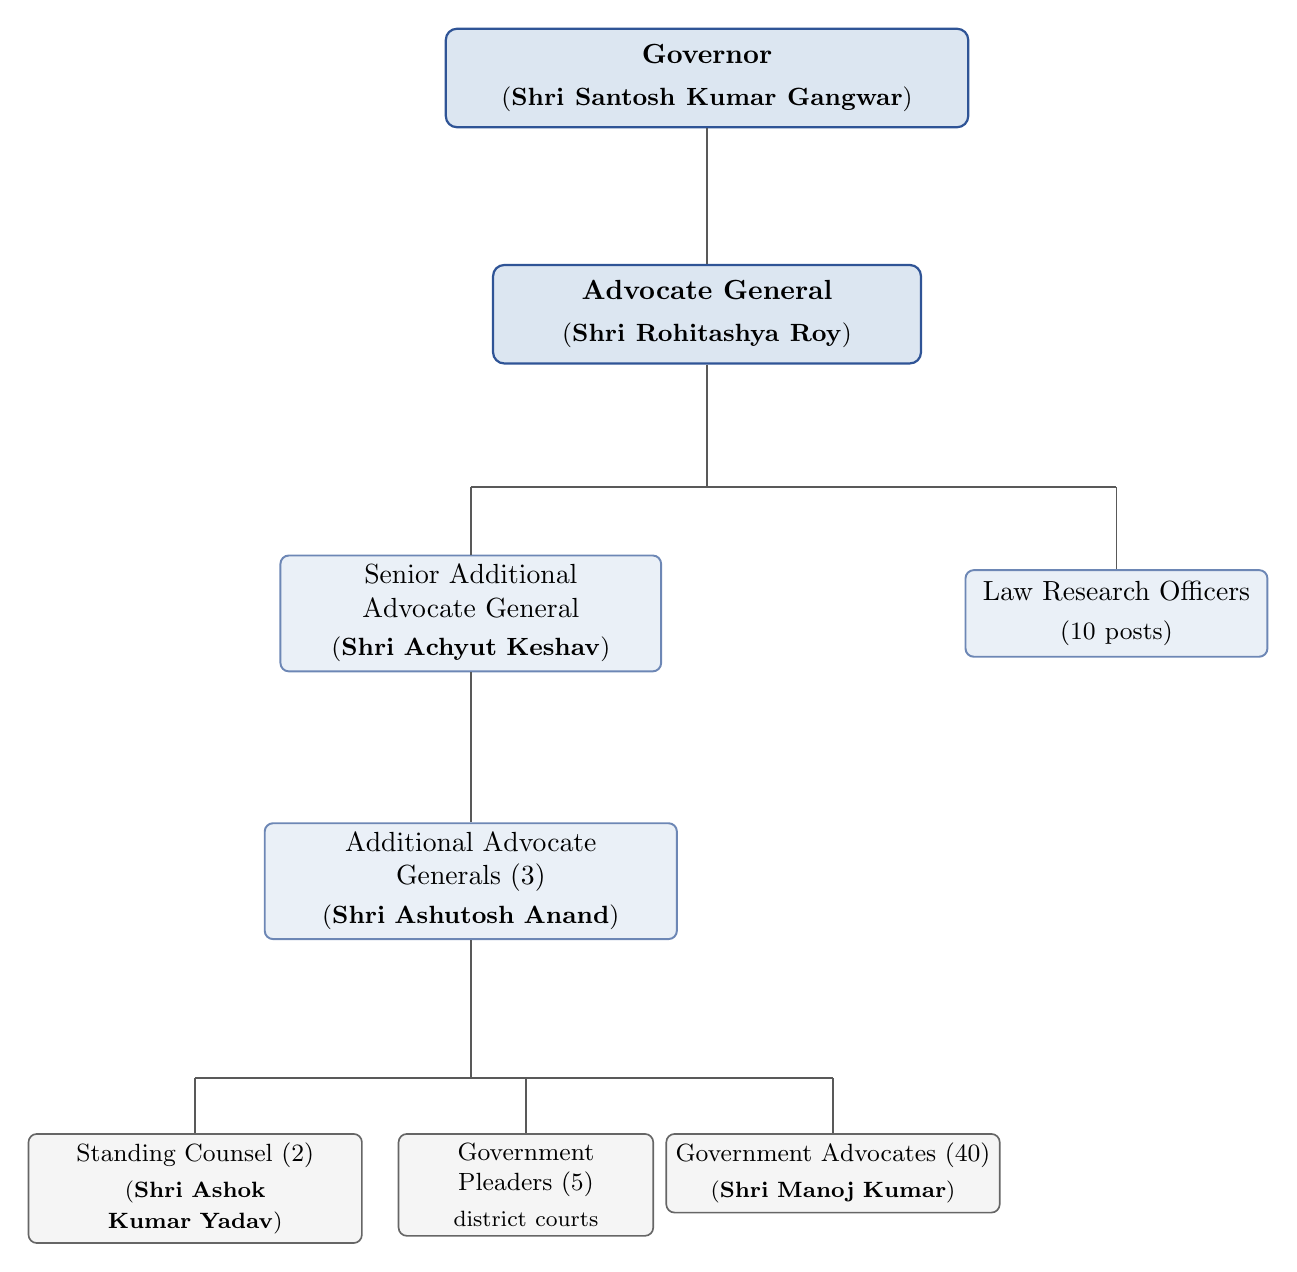
\begin{tikzpicture}
  \node[hroot, text width=6.4cm] (gov) at (0,0)
    {Governor\\[3pt]{\normalfont\small (\textbf{Shri Santosh Kumar Gangwar})}};

  \node[hroot, text width=5.2cm] (ag) at (0,-3.0)
    {Advocate General\\[3pt]{\normalfont\small (\textbf{Shri Rohitashya Roy})}};

  \node[hlvl, text width=4.6cm, font=\normalsize] (saag) at (-3.0,-6.8)
    {Senior Additional Advocate General\\[2pt]{\normalfont\small (\textbf{Shri Achyut Keshav})}};

  \node[hlvl, text width=3.6cm, font=\normalsize] (lro) at (5.2,-6.8)
    {Law Research Officers\\[2pt]{\normalfont\small (10 posts)}};

  \node[hlvl, text width=5.0cm, font=\normalsize] (aag) at (-3.0,-10.2)
    {Additional Advocate Generals (3)\\[2pt]{\normalfont\small (\textbf{Shri Ashutosh Anand})}};

  \node[hleaf, text width=4.0cm, font=\small, anchor=north] (sc) at (-6.5,-13.4)
    {Standing Counsel (2)\\[2pt]{\footnotesize (\textbf{Shri Ashok Kumar Yadav})}};

  \node[hleaf, text width=3.0cm, font=\small, anchor=north] (gp) at (-2.3,-13.4)
    {Government Pleaders (5)\\[2pt]{\footnotesize district courts}};

  \node[hleaf, text width=4.0cm, font=\small, anchor=north] (ga) at (1.6,-13.4)
    {Government Advocates (40)\\[2pt]{\footnotesize (\textbf{Shri Manoj Kumar})}};

  \draw[hlink] (gov.south) -- (ag.north);

  \draw[hlink] (ag.south) -- (0,-5.2);
  \draw[hlink] (-3.0,-5.2) -- (5.2,-5.2);
  \draw[hlink] (-3.0,-5.2) -- (saag.north);
  \draw[hlink] (5.2,-5.2) -- (lro.north);

  \draw[hlink] (saag.south) -- (aag.north);

  \draw[hlink] (aag.south) -- (-3.0,-12.7);
  \draw[hlink] (-6.5,-12.7) -- (1.6,-12.7);
  \draw[hlink] (-6.5,-12.7) -- (sc.north);
  \draw[hlink] (-2.3,-12.7) -- (gp.north);
  \draw[hlink] (1.6,-12.7) -- (ga.north);
\end{tikzpicture}
\end{center}

\noindent{\footnotesize Posts sanctioned in the Office of the Advocate General under the Jharkhand Law Officer (Engagement) Rules, 2026; names as of September 2026.}

% ============================================================= Council of Ministers
\newpage
\section*{Council of Ministers}

\begin{center}
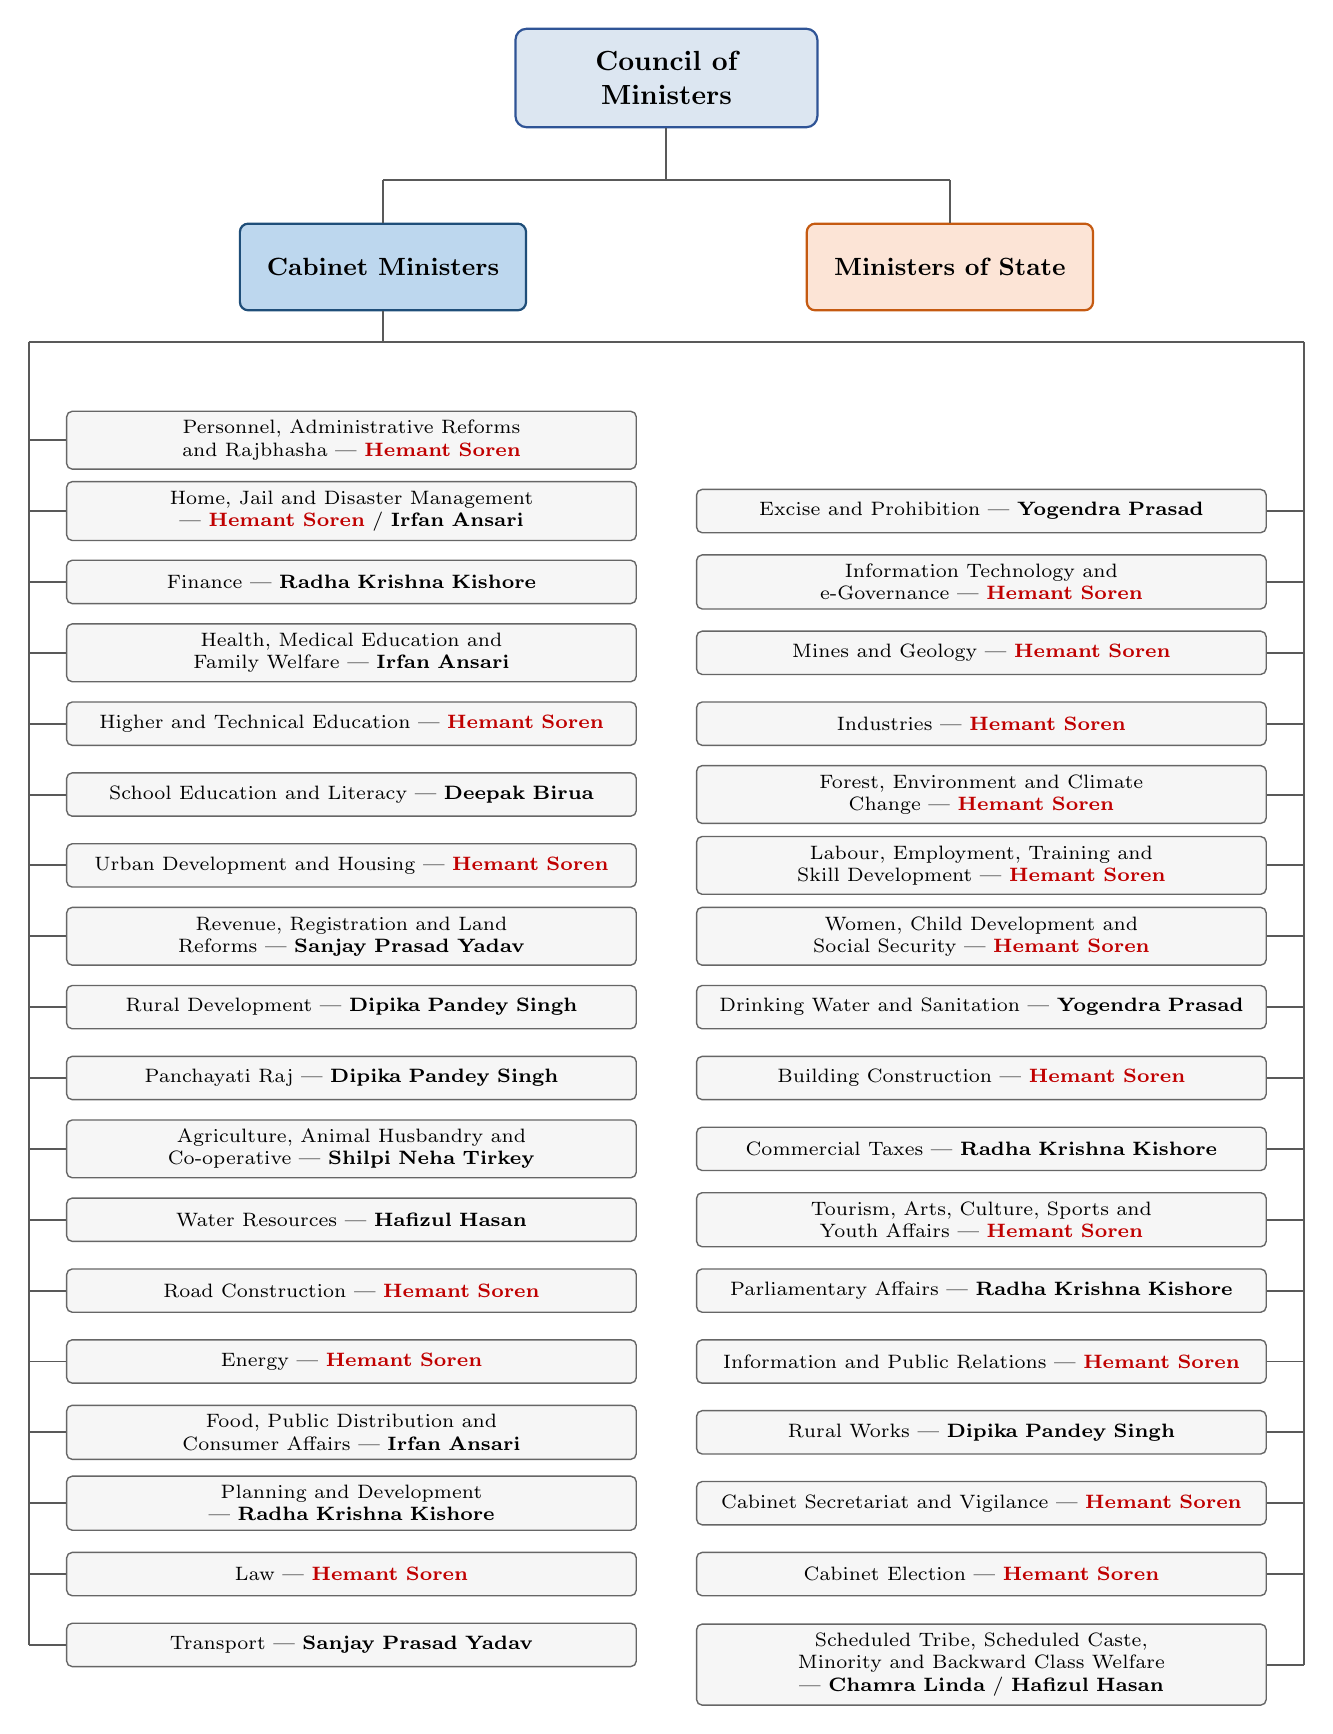
\begin{tikzpicture}
  \node[hroot] (com) at (0,0) {Council of Ministers};

  \node[cabbox] (cab) at (-3.6,-2.4) {Cabinet Ministers};
  \node[mosbox] (mos) at (3.6,-2.4) {Ministers of State};

  % \node[hsub, anchor=north, text width=5.4cm] (charge) at (3.6,-3.7)
  %   {Independent charge or attached\\to a Cabinet Minister};

  \draw[hlink] (com.south) -- (0,-1.3);
  \draw[hlink] (-3.6,-1.3) -- (3.6,-1.3);
  \draw[hlink] (-3.6,-1.3) -- (cab.north);
  \draw[hlink] (3.6,-1.3) -- (mos.north);
  % \draw[hlink] (mos.south) -- (charge.north);

  \draw[hlink] (cab.south) -- (-3.6,-3.35);
  \draw[hlink] (-8.1,-3.35) -- (8.1,-3.35);
  \draw[hlink] (-8.1,-3.35) -- (-8.1,-19.9);
  \draw[hlink] (8.1,-3.35) -- (8.1,-20.15);

  \foreach \nm [count=\i from 0] in {%
    {Personnel, Administrative Reforms and Rajbhasha --- \textbf{\textcolor{cmred}{Hemant Soren}}},%
    {Home, Jail and Disaster Management --- \textbf{\textcolor{cmred}{Hemant Soren}} / \textbf{Irfan Ansari}},%
    {Finance --- \textbf{Radha Krishna Kishore}},%
    {Health, Medical Education and Family Welfare --- \textbf{Irfan Ansari}},%
    {Higher and Technical Education --- \textbf{\textcolor{cmred}{Hemant Soren}}},%
    {School Education and Literacy --- \textbf{Deepak Birua}},%
    {Urban Development and Housing --- \textbf{\textcolor{cmred}{Hemant Soren}}},%
    {Revenue, Registration and Land Reforms --- \textbf{Sanjay Prasad Yadav}},%
    {Rural Development --- \textbf{Dipika Pandey Singh}},%
    {Panchayati Raj --- \textbf{Dipika Pandey Singh}},%
    {Agriculture, Animal Husbandry and Co-operative --- \textbf{Shilpi Neha Tirkey}},%
    {Water Resources --- \textbf{Hafizul Hasan}},%
    {Road Construction --- \textbf{\textcolor{cmred}{Hemant Soren}}},%
    {Energy --- \textbf{\textcolor{cmred}{Hemant Soren}}},%
    {Food, Public Distribution and Consumer Affairs --- \textbf{Irfan Ansari}},%
    {Planning and Development --- \textbf{Radha Krishna Kishore}},%
    {Law --- \textbf{\textcolor{cmred}{Hemant Soren}}},%
    {Transport --- \textbf{Sanjay Prasad Yadav}}%
  }{%
    \pgfmathsetmacro{\yy}{-4.6-0.9*\i}%
    \node[minbox, text width=7.0cm, minimum height=0.55cm] (a\i) at (-4.0,\yy) {\nm};%
    \draw[hlink] (-8.1,\yy) -- (a\i.west);%
  }

  \foreach \nm [count=\i from 0] in {%
    {Excise and Prohibition --- \textbf{Yogendra Prasad}},%
    {Information Technology and \mbox{e-Governance} --- \textbf{\textcolor{cmred}{Hemant Soren}}},%
    {Mines and Geology --- \textbf{\textcolor{cmred}{Hemant Soren}}},%
    {Industries --- \textbf{\textcolor{cmred}{Hemant Soren}}},%
    {Forest, Environment and Climate Change --- \textbf{\textcolor{cmred}{Hemant Soren}}},%
    {Labour, Employment, Training and Skill Development --- \textbf{\textcolor{cmred}{Hemant Soren}}},%
    {Women, Child Development and Social Security --- \textbf{\textcolor{cmred}{Hemant Soren}}},%
    {Drinking Water and Sanitation --- \textbf{Yogendra Prasad}},%
    {Building Construction --- \textbf{\textcolor{cmred}{Hemant Soren}}},%
    {Commercial Taxes --- \textbf{Radha Krishna Kishore}},%
    {Tourism, Arts, Culture, Sports and Youth Affairs --- \textbf{\textcolor{cmred}{Hemant Soren}}},%
    {Parliamentary Affairs --- \textbf{Radha Krishna Kishore}},%
    {Information and Public Relations --- \textbf{\textcolor{cmred}{Hemant Soren}}},%
    {Rural Works --- \textbf{Dipika Pandey Singh}},%
    {Cabinet Secretariat and Vigilance --- \textbf{\textcolor{cmred}{Hemant Soren}}},%
    {Cabinet Election --- \textbf{\textcolor{cmred}{Hemant Soren}}}%
  }{%
    \pgfmathsetmacro{\yy}{-5.5-0.9*\i}%
    \node[minbox, text width=7.0cm, minimum height=0.55cm] (b\i) at (4.0,\yy) {\nm};%
    \draw[hlink] (8.1,\yy) -- (b\i.east);%
  }

  \node[minbox, text width=7.0cm, minimum height=0.55cm] (bw) at (4.0,-20.15)
    {Scheduled Tribe, Scheduled Caste, Minority and Backward Class Welfare
     --- \textbf{Chamra Linda} / \textbf{Hafizul Hasan}};
  \draw[hlink] (8.1,-20.15) -- (bw.east);
\end{tikzpicture}
\end{center}

\noindent{\scriptsize Portfolios as of September 2026.\quad \textcolor{cmred}{\textbf{Red}} = held directly by the Chief Minister.}

\newpage
\section*{Cabinet Ministers and Ministers of State: Difference and Functions}

\noindent{\footnotesize
\renewcommand{\arraystretch}{1.28}%
\begin{tabularx}{\textwidth}{@{}>{\raggedright\arraybackslash}p{3.0cm} >{\raggedright\arraybackslash}X >{\raggedright\arraybackslash}X@{}}
\toprule
 & \textbf{Cabinet Minister} & \textbf{Minister of State} \\
\midrule
Position & Senior minister of Cabinet rank; normally heads a ministry and sits in the Cabinet. & Junior minister below Cabinet rank; assists a Cabinet Minister or holds independent charge of a ministry. \\
\addlinespace[3pt]
Appointment & Appointed by the Governor on the advice of the Chief Minister; must be, or become within six months, a member of either House. & Same manner of appointment and the same membership requirement. \\
\addlinespace[3pt]
Cabinet meetings & Attends Cabinet meetings and shares in collective decisions. & Does not attend Cabinet meetings unless specially invited. \\
\addlinespace[3pt]
Functions & Formulates policy for the ministry, decides its business, supervises the departments and answers for the ministry in the legislature. & Looks after the subjects assigned, assists the Cabinet Minister, represents the ministry in the House; with independent charge, administers the ministry within Cabinet policy. \\
\addlinespace[3pt]
Responsibility & Bound by collective responsibility (Art.~164(2)); answerable for the whole ministry. & Bound by collective responsibility; answerable for the allotted work. \\
\bottomrule
\end{tabularx}}

\vspace{4pt}
\noindent{\footnotesize\textbf{How they function.} The Cabinet Minister sets policy and takes decisions for the ministry; the Minister of State executes the allotted part, coordinates with the departmental secretaries and carries the ministry's case in the House. Both work through the same secretaries, and the Cabinet Minister remains answerable for the ministry as a whole.}

\end{document}
